The main idea of logistic regression is to predict from a set of discrete binary values (ex: have cancer or not [0, 1]). In order to acomplish that, we use a linear function (Decision boundary, can be non-linear) to map all predictions greater than 0.5 as 1 and all less than 0.5 as a 0. This \textbf{prediction} is done by a \textbf{sigmoid} ($g(x)$) function that normalizes the output of the \textbf{Decision boundary} ($\theta^Tx$) to just 1 or 0.

So in conclusion, there is a \textbf{hypotheses} ($h_{\theta}(x)$) function that is the sigmoid ($g(x)$) function applied to the Decision boundary; and the \textbf{goal} is to find the most accurate parameters for the Decision boundary ($\theta^Tx$).

\subsection{Components}
\subsubsection{Sigmoid function}
Also called \textit{Logistic function}, maps any real number to the (0, 1) interval, making it useful for transforming an arbitrary-valued function into a function better suited for classification. The function has this form:

\begin{align}
	g(z) & = \frac{1}{1 + e^{-z}}
\end{align}

And looks like:
\begin{figure}[h]
    \centering
    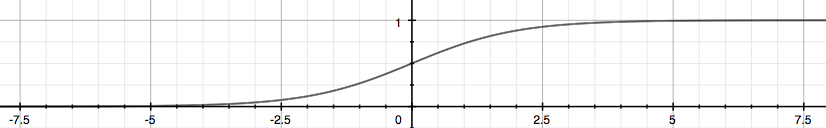
\includegraphics[width=1\textwidth]{sigmoid-function}
    \caption{Sigmoid function}
    \label{fig:sigmoid}
\end{figure}

\subsubsection{Hypotheses function}
This hypotheses function will predict, using some input data ($x_i$) and a set of precomputed coefficients ($\theta$), a number between 0 and 1.

$$0 \le h_{\theta}(x) \le 1$$

In order to achieve this, we use the sigmoid function to map our output to 0 - 1 interval on the decision boundary. The function has this form:

\begin{align}
	h_{\theta}(x) & = g(\theta^Tx) \\
	h_{\theta}(x) & = \frac{1}{1 + e^{-\theta^Tx}}
\end{align}

The result of this function can be interpreted as \textit{the probability that the output is 1}. For example, $h_{\theta}(x)=0.7$ gives us a probability of 70\% that our output is 1. Our probability that our prediction is 0 is just the complement of our probability that it is 1 (e.g. if probability that it is 1 is 70\%, then the probability that it is 0 is 30\%).


\subsubsection{Decision boundary}